\begin{definition}[Edge-cut]
  An \textit{edge-cut} in a graph \(G\) is a set \(X\) of edges
  in \(G\) such that \(G \setminus X\) is disconnected. An
  edge-cut of minimum cardinality is called a minimum edge-cut.
\end{definition}

\begin{definition}[Edge-connectivity]
  The \textit{edge-connectivity}, denoted by \(\lambda(G)\), is
  the cardinality of a minimum edge-cut. In addition, a graph is
  said to be \(k\)-edge-connected if \(\lambda(G) \geq k\).
\end{definition}

\begin{nexample}
  \(\lambda(C_n) = 2\) and \(\lambda(K_n) = n-1\).
\end{nexample}

\begin{figure}[ht]
\begin{nexample}
  Following are examples of graphs \(G\) with the following
  properties:
  \begin{enumerate}
    \item \(\kappa(G) = 1, \lambda(G) = 1, \delta(G) = 1\)
      \begin{center}
        
\includegraphics[width=0.39\textwidth]{figures/l10/props1}
      \end{center}

    \item \(\kappa(G) = 1, \lambda(G) = 1, \delta(G) = 10\)
      \begin{center}
        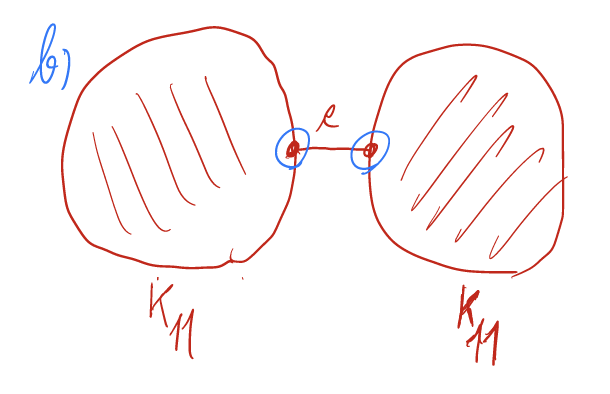
\includegraphics[width=0.39\textwidth]{figures/l10/props2}
      \end{center}

    \item \(\kappa(G) = 1, \lambda(G) = 10, \delta(G) = 10\)
      \begin{center}
        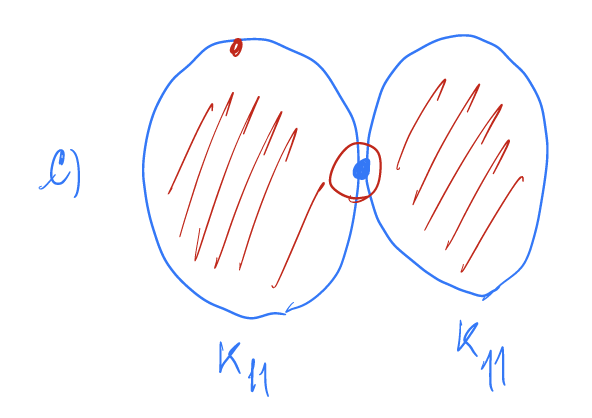
\includegraphics[width=0.39\textwidth]{figures/l10/props3}
      \end{center}
  \end{enumerate}
\end{nexample}
\end{figure}

\begin{theorem}
  For every graph \(G\), 
  \begin{displaymath}
    \kappa(G) \leq \lambda(G) \leq \delta(G)
  \end{displaymath}
\end{theorem}

\begin{proof}
  % First, we will show that \(\lambda(G) \leq \delta(G)\). Let
  % \(v\) be a vertex of \(G\) with minimum degree \(\delta(G)\).
  % Notice that the edges incident to \(v\) is an edge-cut of
  % \(G\)..

  % Now, we will show that \(\kappa(G) \leq \lambda(G)\). Let
  % \(U\) be the set of vertices in \(G\) that are adjacent to an
  % edge-cut \(X\). Then, removing every edge in \(U\) would result
  % in a disconnected graph.

  Requires re-write due to informal in-class proof.
\end{proof}

\begin{theorem}
  If \(G\) is a cubic (3-regular) graph, then \(\kappa(G) =
  \lambda(G)\).
\end{theorem}

\begin{proof}
  We will consider the possible values of \(\kappa(G): \{0, 1, 2,
  3\}\).
  \begin{enumerate}[label=(\alph*.)]
    \item When \(\kappa(G) = 0\), the graph is disconnected so
      \(\lambda(G) = 0\) as well.
    \item When \(\kappa(G) = 1\), then there is a cut-vertex.
      Then, one of the edges incident to the cut-vertex must be a
      bridge and removing that edge makes the graph disconnected.
    \item When \(\kappa(G) = 2\), then there are two vertices in
      the vertex-cut. We can then apply the same reasoning as
      above and we would have \(\lambda(G) = 2\).
    \item When \(\kappa(G) = 3\), then \(\lambda(G) = 3\) since
      since \(3 = \kappa(G) \leq \lambda(G) \leq \delta(G) = 3\)
      by previous theorem.
  \end{enumerate}
\end{proof}

\begin{theorem}
  If \(G\) is a graph of order \(n\) and size \(m \geq n-1\),
  then 
  \begin{displaymath}
    \kappa(G) \leq \left\lfloor\frac{2m}{n}\right\rfloor
  \end{displaymath}
\end{theorem}

\begin{proof}
  Recall that
  \[
    \sum_{v \in V(G)} \deg v = 2m \qquad \text{and} 
    \qquad \sum_{v \in V(G)} \deg v \geq n \cdot \delta(G) 
  \]
  With these two, we would have that 
  \[
    2m \geq n \cdot \delta(G) \qquad \text{and}
    \qquad \left\lfloor \frac{2m}{n} \right\rfloor \geq \delta(G) 
  \]
  Then, we would have that 
  \[
    \left\lfloor \frac{2m}{n} \right\rfloor \geq \delta(G) \geq
    \kappa(G) 
  \]
\end{proof}

\section{Menger's Theorem}

\begin{theorem}[Menger, 1927]
  Let \(u\) and \(v\) be non-adjacent vertices in a graph \(G\).
  The minimum number of vertices in a \(u-v\) separating set
  equals the maximum number of internally disjoint \(u-v\) paths
  in \(G\).
\end{theorem}

\begin{proof}
  I give up.
  \href{https://youtu.be/2rbbq-Mk-YE?si=C78wD7AtOfpNnipF}{Watch
  this video.}
\end{proof}

\begin{nexample}
  Use Menger's Theorem to show that any two vertices of a
  2-connected graph lie on a common cycle.

  Recall that a 2-connected graph means that we need to remove at
  least 2 vertices to disconnect the graph. This means that given
  any \(u, v \in V(G)\), there are two paths joining them. By
  Menger's Theorem, if there are two disjoint paths \(P_1, P_2\)
  and \(P_1 \cup P_2\) forms a cycle.
\end{nexample}

\begin{theorem}[Menger's Theorem: Edge Version]
  For distinct vertices \(u, v\) in a graph \(G\), the minimum
  number of edges of \(G\) that separate \(u\) and \(v\) equals
  the maximum number of pair-wise edge-disjoint \(u-v\) paths in
  \(G\).
\end{theorem}

